
\documentclass{article}
\usepackage[ascii]{inputenc}
\usepackage[T1]{fontenc}
\usepackage[english]{babel}
\usepackage{amsmath}
\usepackage{amssymb,amsfonts,textcomp}
\usepackage{color}
\usepackage{array}
\usepackage{supertabular}
\usepackage{hhline}
\usepackage[normalem]{ulem}
\usepackage{hyperref}
\usepackage{textcomp}
\usepackage{layout}
\usepackage[numbers]{natbib}
\usepackage{caption}
\usepackage{subcaption}
\usepackage{enumerate}
\usepackage[table]{xcolor}
\definecolor{light-gray}{gray}{0.8}
\definecolor{light-light-gray}{gray}{0.9}

\hypersetup{colorlinks=true, linkcolor=black, citecolor=black, filecolor=blue, urlcolor=blue, pdftitle=CAD20abstract, pdfauthor=Orest Mykhaskiv, pdfsubject=, pdfkeywords=}
\usepackage[pdftex]{graphicx}

\newcommand\textstyleInternetlink[1]{\textcolor{blue}{#1}}

\setcounter{secnumdepth}{2}
\renewcommand\thesection{\arabic{section}}
\renewcommand\thesubsection{\arabic{section}.\arabic{subsection}}
\makeatletter
\newcommand\arraybslash{\let\\\@arraycr}
\makeatother

\newcommand\liststyleWWviiiNumxxxiii{%
\renewcommand\labelitemi{{\textbullet}}
\renewcommand\labelitemii{{}-}
\renewcommand\labelitemiii{${\blacksquare}$}
\renewcommand\labelitemiv{{\textbullet}}
}
\newcommand\liststyleWWviiiNumxxix{%
\renewcommand\labelitemi{{\textbullet}}
\renewcommand\labelitemii{o}
\renewcommand\labelitemiii{${\blacksquare}$}
\renewcommand\labelitemiv{{\textbullet}}
}
\newcommand\liststyleWWviiiNumxxiv{%
\renewcommand\labelitemi{{\textbullet}}
\renewcommand\labelitemii{o}
\renewcommand\labelitemiii{${\blacksquare}$}
\renewcommand\labelitemiv{{\textbullet}}
}
\newcommand\liststyleWWviiiNumxxi{%
\renewcommand\labelitemi{{\textbullet}}
\renewcommand\labelitemii{o}
\renewcommand\labelitemiii{${\blacksquare}$}
\renewcommand\labelitemiv{{\textbullet}}
}
\newcommand\liststyleWWviiiNumxxiii{%
\renewcommand\labelitemi{{\textbullet}}
\renewcommand\labelitemii{o}
\renewcommand\labelitemiii{${\blacksquare}$}
\renewcommand\labelitemiv{{\textbullet}}
}
\newcommand\liststyleWWviiiNumxv{%
\renewcommand\labelitemi{{\textbullet}}
\renewcommand\labelitemii{o}
\renewcommand\labelitemiii{${\blacksquare}$}
\renewcommand\labelitemiv{{\textbullet}}
}
\newcommand\liststyleWWviiiNumxxx{%
\renewcommand\theenumi{\arabic{enumi}}
\renewcommand\theenumii{\alph{enumii}}
\renewcommand\theenumiii{\roman{enumiii}}
\renewcommand\theenumiv{\arabic{enumiv}}
\renewcommand\labelenumi{[\theenumi]}
\renewcommand\labelenumii{\theenumii.}
\renewcommand\labelenumiii{\theenumiii.}
\renewcommand\labelenumiv{\theenumiv.}
}
\newcommand\liststyleWWviiiNumxxxii{%
\renewcommand\labelitemi{{\textbullet}}
\renewcommand\labelitemii{o}
\renewcommand\labelitemiii{${\blacksquare}$}
\renewcommand\labelitemiv{{\textbullet}}
}

\renewcommand\refname{}
\renewcommand{\bibsection}{}
\renewcommand{\theequation}{2.\arabic{equation}}


\setlength\paperwidth{19.05cm}
\setlength\paperheight{26.162cm}
\setlength\voffset{-1in}
\setlength\hoffset{-1in}
\setlength\topmargin{30pt}
\setlength\oddsidemargin{1.524cm}
\setlength\textheight{576pt}
\setlength\textwidth{16.001999cm}
\setlength\footskip{0.841cm}
\setlength\headheight{16pt}
\setlength\headsep{28pt}


\usepackage{fancyhdr}
\pagestyle{fancy}
\fancyhf{}
\renewcommand{\headrulewidth}{0pt}
\renewcommand{\footrulewidth}{0.4pt}
\fancyhead[R]{\thepage}
\fancyfoot[R]{Proceedings of CAD'20, Barcelona, Spain, July 6-8, 2020, aaa-bbb\\ {\footnotesize{\textcopyright}} 2020 CAD Solutions, LLC, \ULurl{http://www.cad-conference.net}}

\usepackage{etoolbox}
\patchcmd{\thebibliography}{\section*{\refname}}{}{}{}
\captionsetup[figure]{labelformat={default},name={Fig.}}

\setlength{\bibsep}{2pt plus 0.3ex}
\setcounter{page}{1}

\makeatletter
\DeclareUrlCommand\ULurl@@{%
  \def\UrlFont{\ttfamily\color{blue}}%
  \def\UrlLeft{\uline\bgroup}%
  \def\UrlRight{\egroup}}
\def\ULurl@#1{\hyper@linkurl{\ULurl@@{#1}}{#1}}
\DeclareRobustCommand*\ULurl{\hyper@normalise\ULurl@}
\makeatother

\begin{document}

{\centering  
\includegraphics[width=5.173cm,height=2.193cm]{images/CADconverted-img001.jpg} \par}

\vspace{5pt}
\noindent
\underline{Title:}

\noindent{\bfseries
On the CAD-compatible conversion of multi-sided surfaces}

\vspace{1em}
\noindent \underline{Authors:}
\newline
P\'eter Salvi, salvi@iit.bme.hu, Budapest University of Technology and Economics \newline
Tam\'as V\'arady, varady@iit.bme.hu, Budapest University of Technology and Economics \newline
Alyn Rockwood, alynrock@gmail.com, Boulder Graphics LLC, USA

\vspace{1em}
\noindent \underline{Keywords:}\newline
B\'ezier surface, Trimming, Charrot--Gregory patch, S-patch


\bigskip


\noindent \underline{DOI:} 10.14733/cadconfP.2020.xxx-yyy

\vspace{10pt}
\noindent\underline{Introduction:}\vspace{0.2em}\newline
The majority of aesthetic objects is represented by free-form shapes, and modeling these
naturally involves multi-sided (i.e., non-four-sided) surfaces, as well.  The
mathematical representation of such patches is still an active area in CAGD, and although
a great variety of approaches have been published, none of the genuine $n$-sided
formulations have been standardized so far.

On the other hand, commercial CAD/CAM systems and related application programs only accept
data in standard formats, such as tensor product NURBS surfaces. For this reason, it is a
widely applied practice to convert multi-sided surfaces into a CAD-compatible
representation either by (i)~approximating them with larger quadrilaterals,
\emph{trimming} away the exterior part beyond the boundaries, or (ii)~\emph{splitting}
them into smaller four-sided patches.

Both techniques have their deficiencies. They only approximate the original multi-sided
surface, and trimming -- in general -- cannot ensure even $C^0$ continuity between the
adjacent patches. In the splitting scheme the subdividing curves in the interior
weaken the overall continuity of the surface.

Ideally, we would like to have an $n$-sided patch that:
\begin{enumerate}[i)]
\item can be used for design (has intuitive controls),
\item can be attached to adjacent patches with $G^1$ or higher continuity,
\item and can also be represented \emph{accurately} as a tensor product NURBS surface.
\end{enumerate}

The above problem can be resolved, if the multi-sided surfaces can be represented as rational
polynomials of two parametric variables. Then they can be directly converted into
NURBS form, without either changing the surfaces or harming continuity. The result will be
a collection of \emph{watertight trimmed surfaces} with exact trimming curves.
 
Some of the well-known multi-sided schemes allow computing a trimmed bi-parametric
representation. Our goal in this paper is to review these and discuss the difficulties of
the conversion process. We are going to provide further insights into specific
computational and geometric problems, that have not been discussed elsewhere and are
useful for analyzing the ``pros and cons'' of these representations.
We will investigate four schemes, and show actual high-degree conversion examples with
control grids.
A general discussion will conclude the paper.

\vspace{10pt}
\noindent\underline{S-patch:}\vspace{0.2em}\newline
The S-patch of Loop \& DeRose~\cite{spatch1} is a generalization of the B\'ezier triangle, or,
more precisely, a B\'ezier simplex mapping from $(n-1)$D to 3D, where the $n$ coordinates of the
domain are supplied by generalized barycentric coordinates. The \emph{depth} ($d$) of an S-patch
is the number of deCasteljau steps it takes to evaluate a surface point, i.e., something similar
to the degree of a B\'ezier triangle (but not the degree of the S-patch itself).
S-patches have many nice properties, and are known to be convertable into tensor product
rational B\'ezier surfaces of degree $d(n-2)$.

One drawback of this representation is its large number of control points, which renders it
inconvenient for interactive design. For example, a five-sided patch of depth 5 has 126 control
points, while a 4-sided tensor product patch has only 36. A possible workaround is to use a
$G^1$ \emph{frame} for design that defines the tangent planes at the boundaries.
After increasing the depth by 3, these boundary constraints can be interpolated~\cite{spatch2},
and the remaining interior control points can be set by some heuristic to generate a smooth
surface~\cite{salvi-kepaf}, see the figure below.
\begin{figure}[h!]
  \centering
  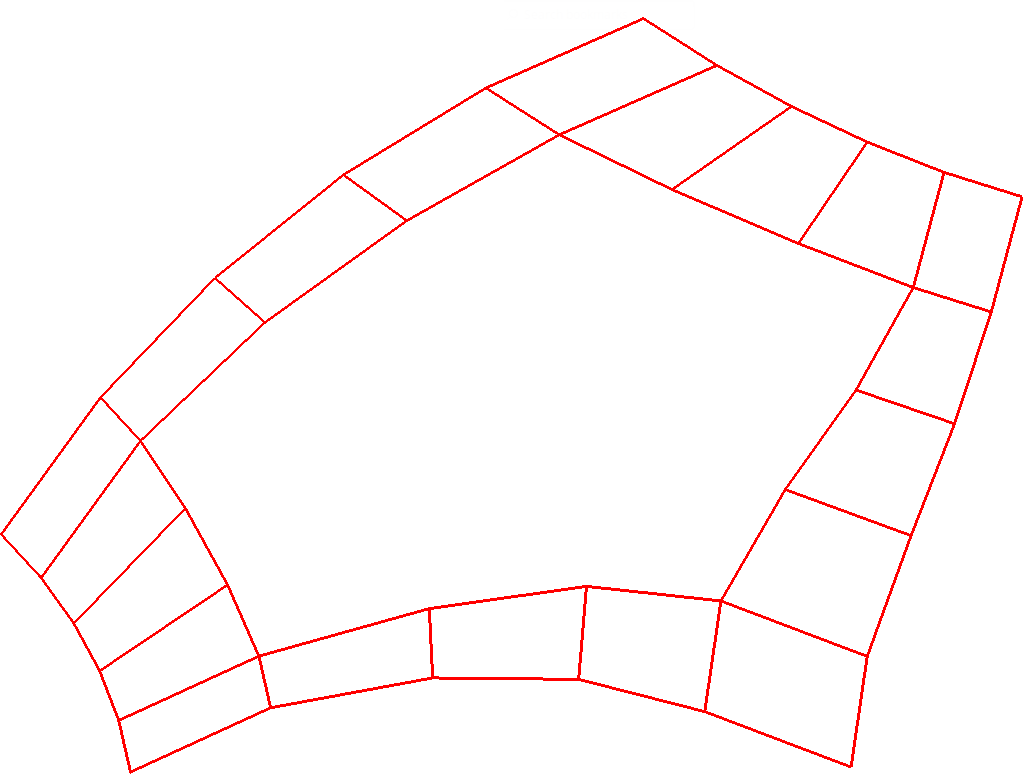
\includegraphics[width = 0.3\textwidth]{images/5-5-bezier-ribbon.png}
  \hfill
  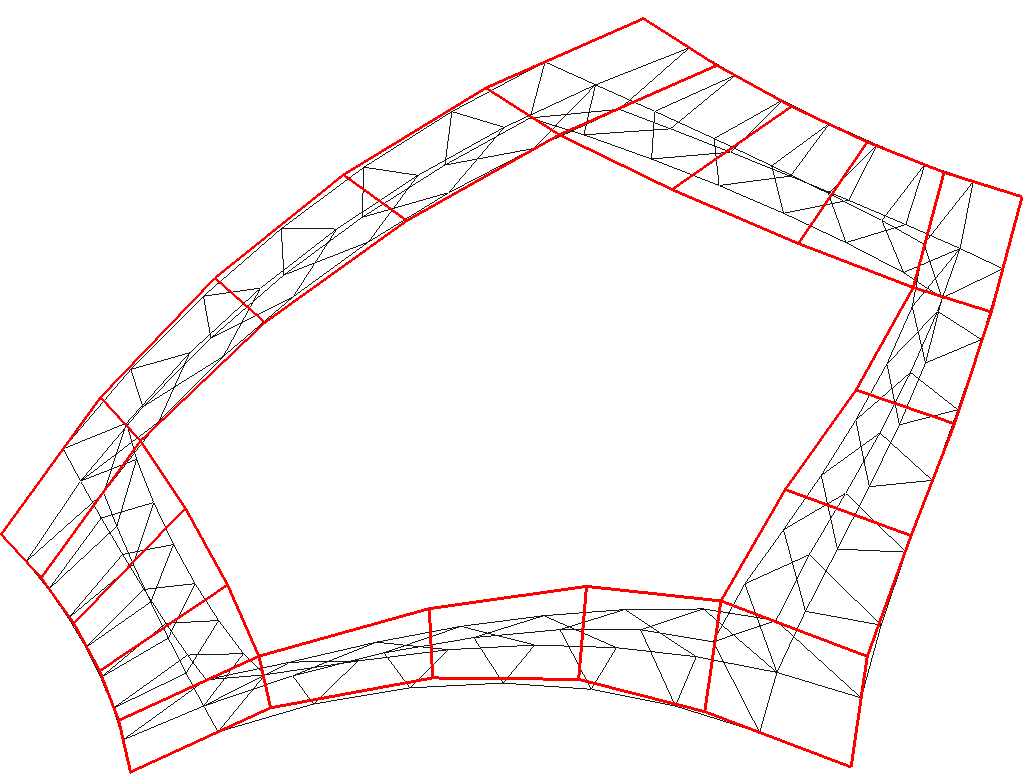
\includegraphics[width = 0.3\textwidth]{images/5-5-cnet-ribbon.png}
  \hfill
  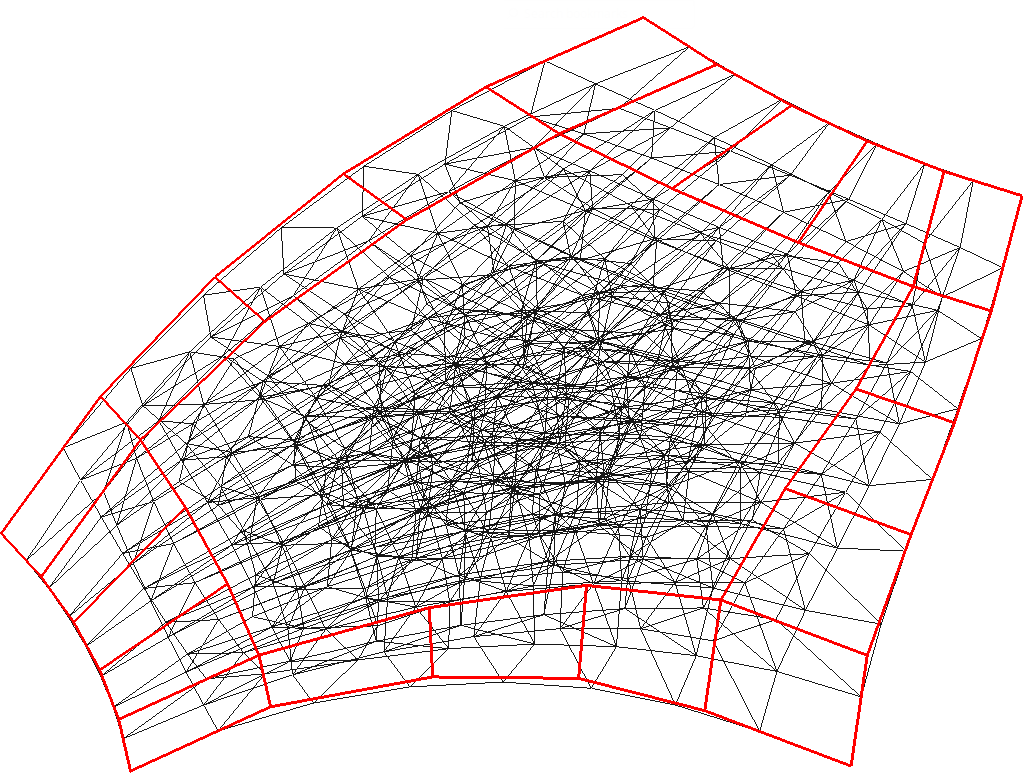
\includegraphics[width = 0.3\textwidth]{images/5-5-cnet-full.png}
\end{figure}

The CAD-compatible conversion presented in~\cite{spatch1} is a two-step process:
first convert the surface into a
four-sided S-patch, and then to a tensor product patch. The first step is based on the
composition of B\'ezier simplexes, which has very high complexity.
Even using an efficient algorithm~\cite{simplex2}, converting a modest-sized S-patch
still requires minutes of computation on today's machines~\cite{salvi-wait}.

Here we propose an alternative conversion process. Since a B\'ezier simplex is just a polynomial,
the only problem is how to express the generalized barycentric coordinates as a rational polynomial
of the $(u,v)$ parameters on the 2D domain. Using Wachspress coordinates over a regular $n$-sided
polygon, the barycentric coordinates $\{\lambda_i\}$ are expressed as
\begin{equation}
  \label{eq:wachspress}
  \lambda_i(u,v) = \prod_{\substack{j=1\\j\notin\{i-1,i\}}}^nh_j(u,v) \quad\bigg/\quad
                   \sum_{k=1}^n\prod_{\substack{j=1\\j\notin\{k-1,k\}}}^nh_j(u,v),
\end{equation}
where the indexing is cyclic, and $h_j(u,v)$ is a distance function
from the $j$-th side of the domain polygon. The implicit
equation of the line containing a given side is suitable for this purpose,
and is also a linear polynomial,
so the Wachspress coordinates can be expressed as rational polynomials of degree $n-2$. We
normalize the distances such that they take on the value 1 at vertices adjacent to the side.

With this method, the B\'ezier control points of the tensor product representation
can be located by straightforward computation, which takes only milliseconds.

\vspace{10pt}
\noindent\underline{Warren's patch:}\vspace{0.2em}\newline
Warren~\cite{warren} created multi-sided patches from B\'ezier triangles by assigning $0/0$
\emph{base points} to some of the control points, essentially cutting off the corners, and thus
creating 5- and 6-sided surfaces. A simple conversion to a (degenerate) tensor product form is
also shown in the paper.

A nice property of this patch is that the ``remaining'' control points define the behavior of the
boundary in the same way as in a normal B\'ezier triangle, i.e., the first control row defines
its position as a B\'ezier curve, the second its first derivatives etc.
The figure below shows the creation of a 5-sided patch and its conversion.
\begin{figure}[h!]
  \centering
  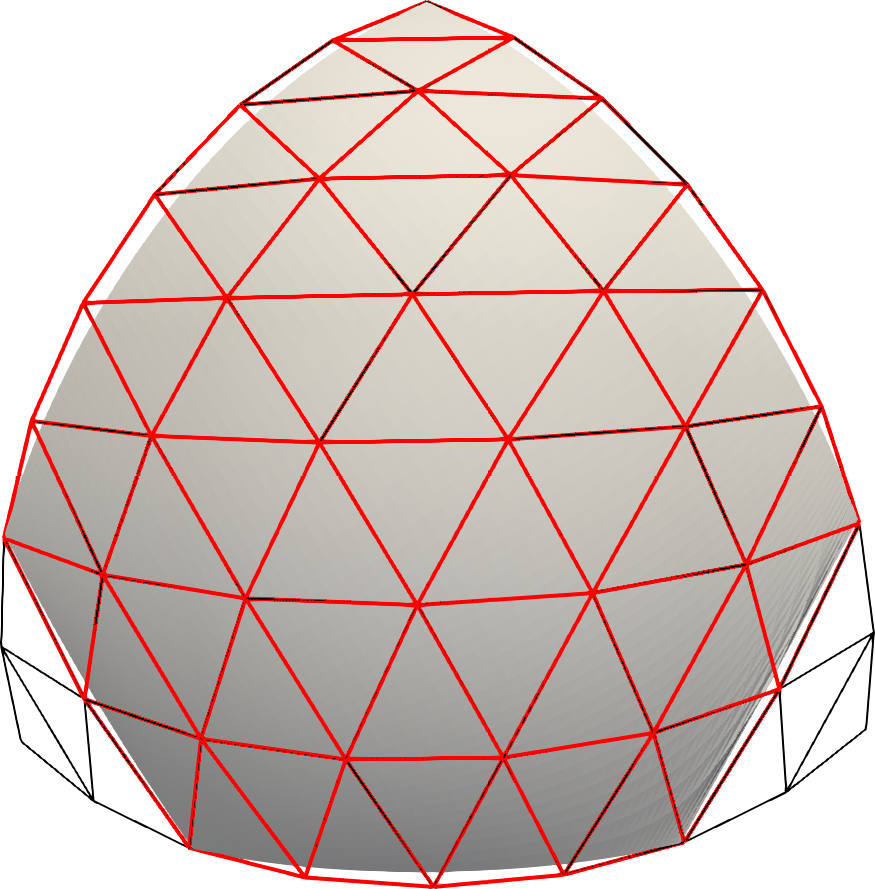
\includegraphics[width = 0.20\textwidth]{images/warren-cnet.png}
  \hspace{3cm}
  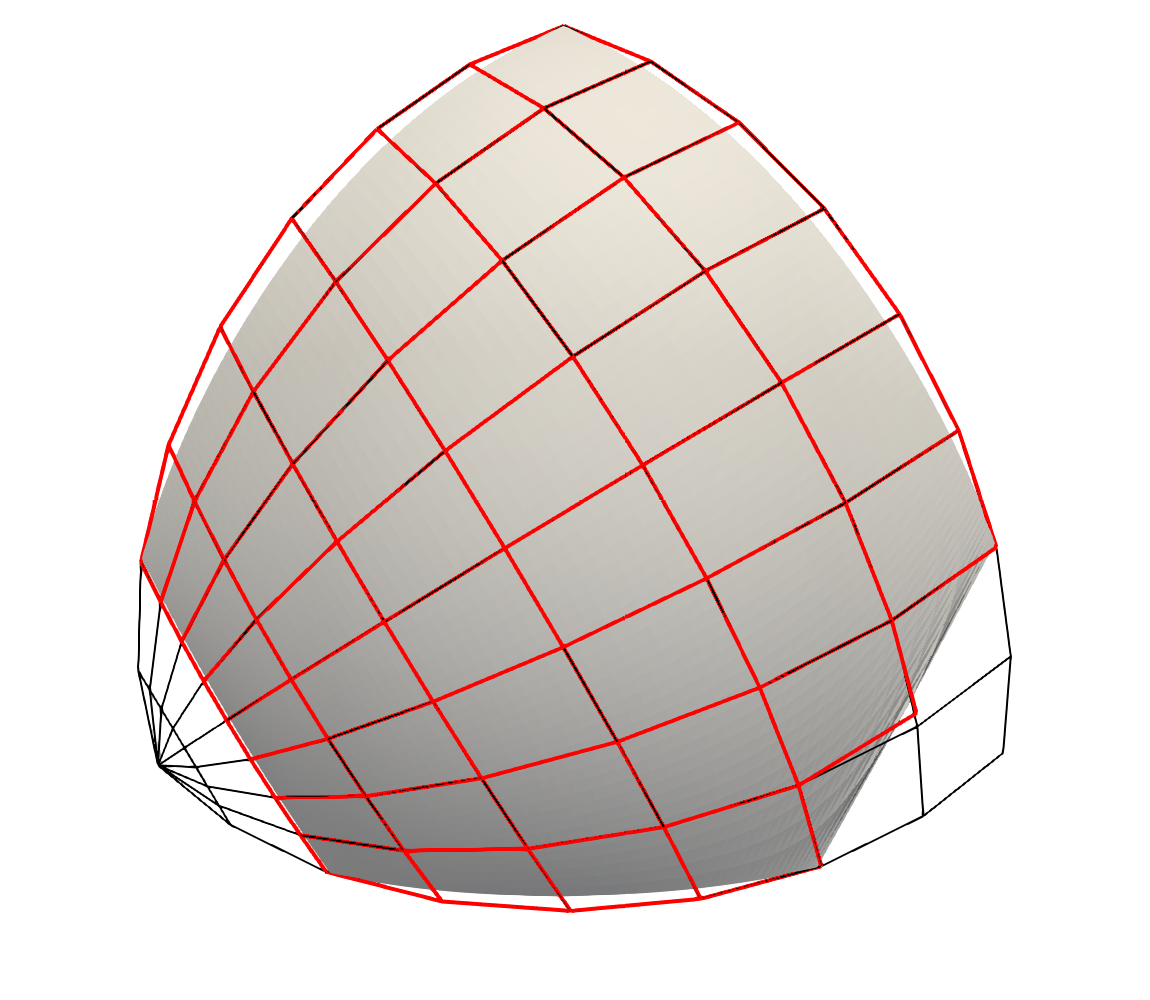
\includegraphics[width = 0.20\textwidth]{images/warren-quad.png}
\end{figure}

Note, however, that not all degree configurations are available. A 6-sided patch with degree-$d$
boundaries can be created from a triangle of degree $3d$, but due to its asymmetric construction,
a 5-sided patch cannot have boundaries of the same degree. Moreover, using control points with zero
weight is not a standard practice, and is not supported by many systems. Meshing
also presents a problem, as a uniform grid on the domain would result in distorted triangles
(the ``trimmed'' sides correspond to corners).

% Toric patches ...

\vspace{10pt}
\noindent\underline{Kato's patch:}\vspace{0.2em}\newline
Kato~\cite{kato} proposed a surface defined as the transfinite interpolation of boundary curves with
cross-derivatives. When these boundary constraints are given as a $G^1$ frame (and hence
are polynomial), the whole patch may become polynomial. The tricky part is the parameterization:
this representation uses two local parameters, a \emph{side parameter} $s_i$
that takes on values from 0 to 1 as it sweeps from one adjacent side to the other,
and a \emph{distance parameter} $h_i$ that vanishes on the base side $i$, see
Figure~\ref{fig:parameters}.
\begin{figure}[b!]
  \begin{subfigure}{0.30\textwidth}
    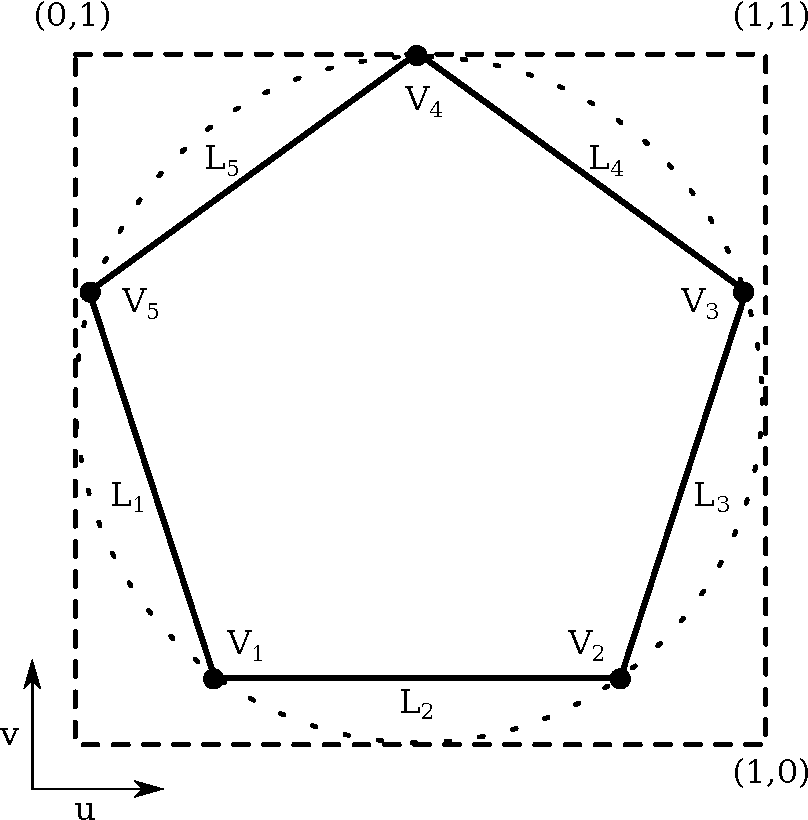
\includegraphics[width = \textwidth]{images/domain.pdf}
    \caption{Domain}
    \label{fig:domain}
  \end{subfigure}
  \hfill
  \begin{subfigure}{0.3\textwidth}
    \begin{minipage}[b][5cm][b]{\textwidth}
      \centering
      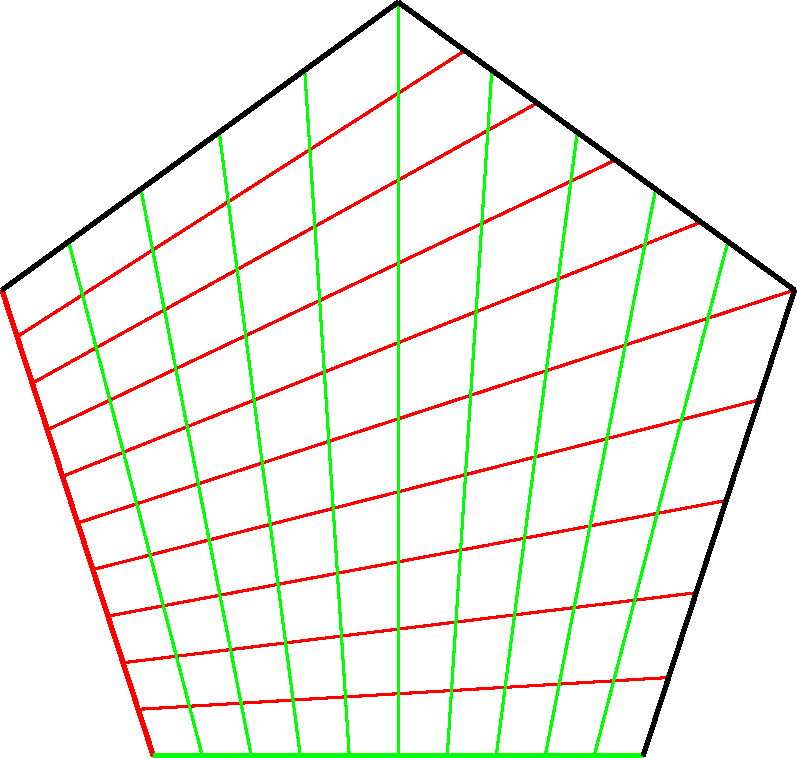
\includegraphics[width = \textwidth]{images/s-params.pdf}
      \vspace*{-2mm}
    \end{minipage}
    \caption{$s_i$ isolines for two sides}
    \label{fig:s}
  \end{subfigure}
  \hfill
  \begin{subfigure}{0.30\textwidth}
    \begin{minipage}[b][5cm][b]{\textwidth}
      \centering
      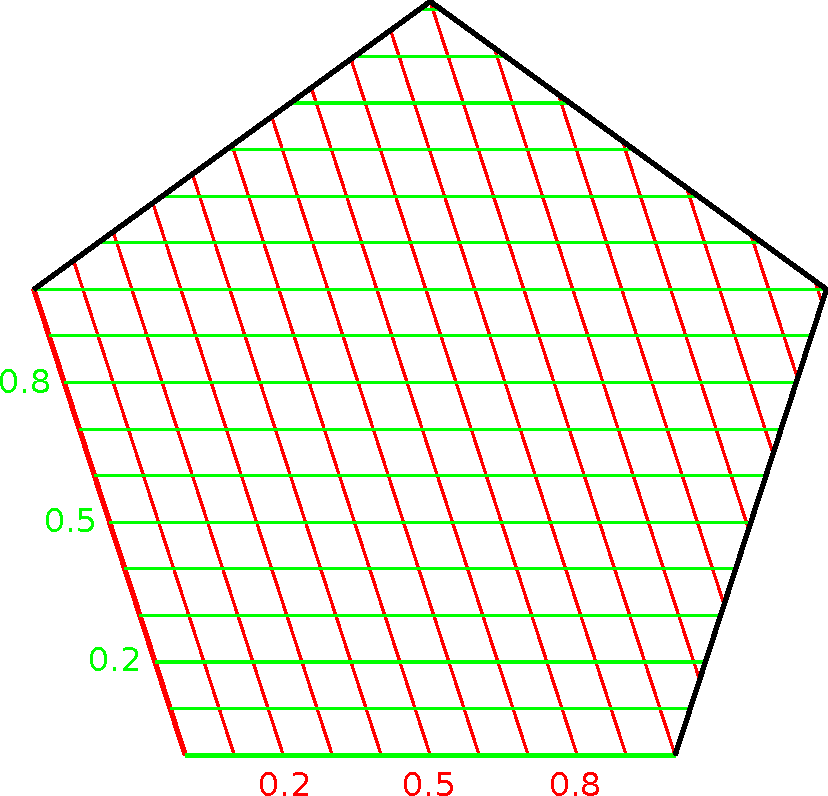
\includegraphics[width = \textwidth]{images/h-params.pdf}
      \vspace*{-2mm}
    \end{minipage}
    \caption{$h_i$ isolines for two sides}
    \label{fig:h}
  \end{subfigure}
  \caption{Parameterization.}
  \label{fig:parameters}
\end{figure}

The distance parameters can be computed the same way as in the creation of S-patches, and for side
parameters we can use $s_i=h_{i-1}/(h_{i-1}+h_{i+1})$, which gives a rational polynomial
representation.

Kato's patch is easily extendable to handle $G^2$ continuity, if the side constraints have 3
control rows (so the cross-degree $d^\perp$ is 2 instead of 1).
Then the whole surface becomes a rational tensor product B\'ezier patch of
degree $nd+(n-1)(d^\perp+1)+d^\perp$.

\vspace{10pt}
\noindent\underline{Charrot--Gregory patch:}\vspace{0.2em}\newline
The same idea can be used to convert Charrot--Gregory patches~\cite{charrot} that use
only side parameters. (Note that on a regular domain the $s_i$ parameters defined above
will be the same as the radial parameterization in the original paper.)
The input is given as a $G^1$ frame; the converted patch is of degree $nd+2(n-2)$.

For triangular surfaces, we can use the $h_{i-1}$ parameter as a side parameter for the $i$-th
side instead of $s_i$, thereby reducing the overall degree to $d+3$.
An example of four watertight trimmed patches with contours, mean curvature
and isophote lines is shown below.
\begin{figure}[h!]
  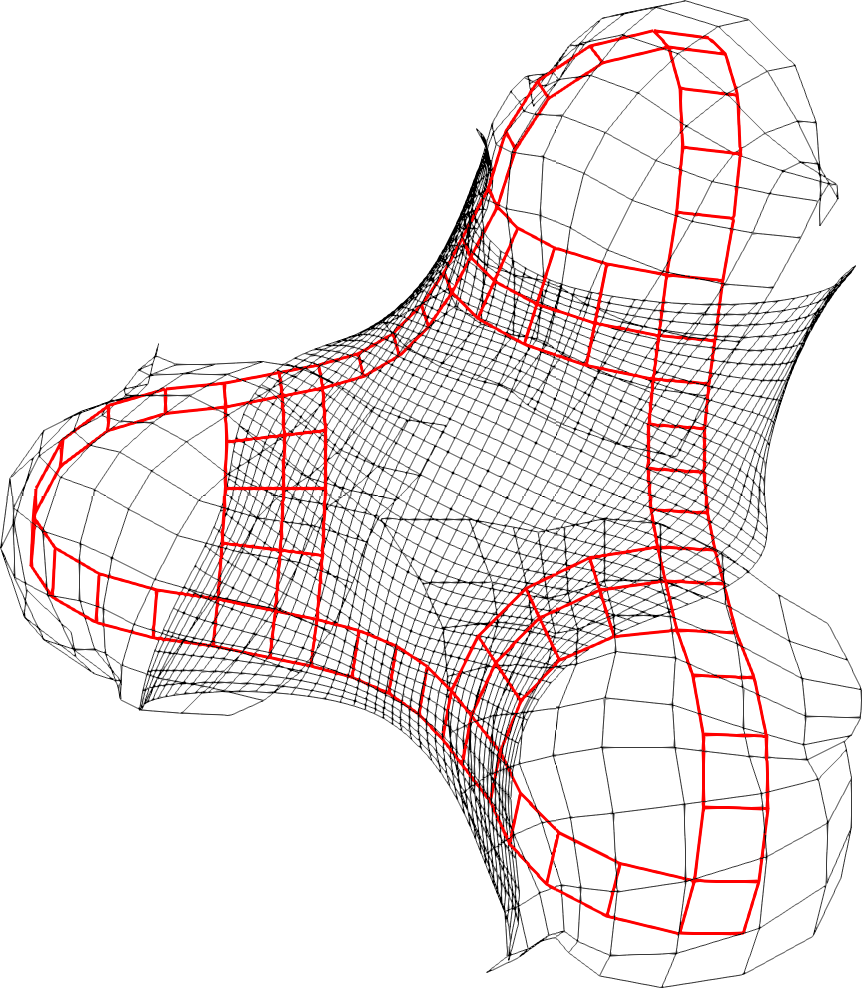
\includegraphics[width = 0.2139\textwidth]{images/trebol3-cnet.png}
  \hfill
  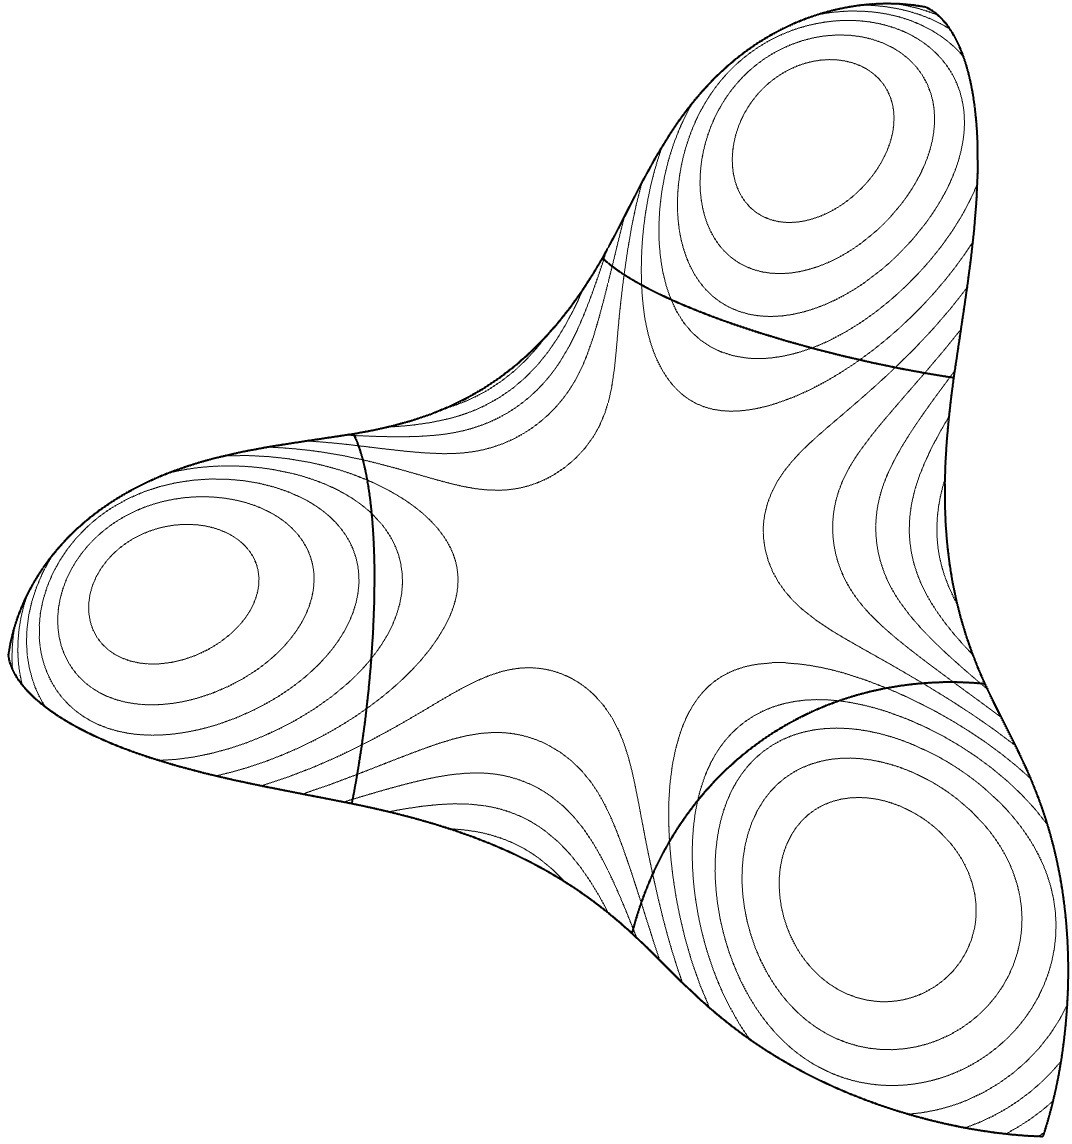
\includegraphics[width = 0.23\textwidth]{images/trebol3-contour.jpg}
  \hfill
  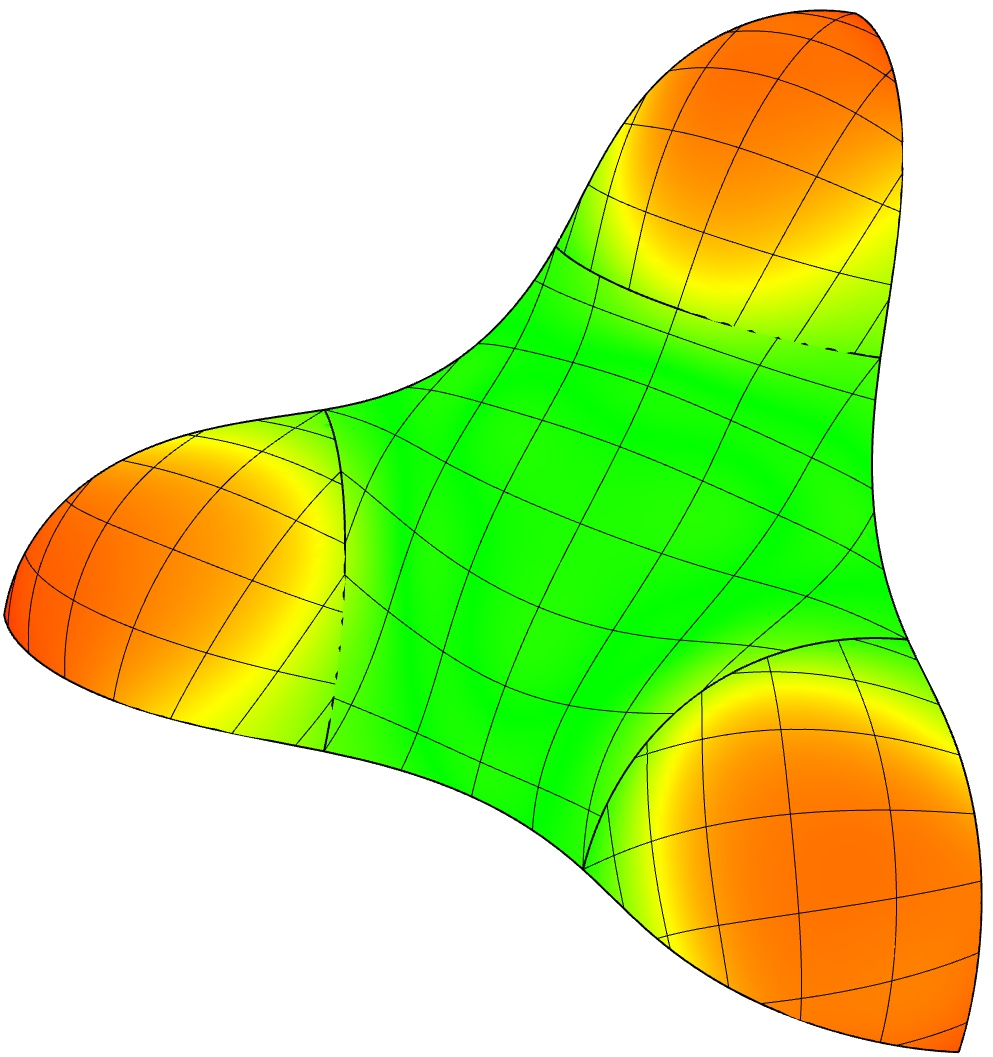
\includegraphics[width = 0.23\textwidth]{images/trebol3-mean-iso.jpg}
  \hfill
  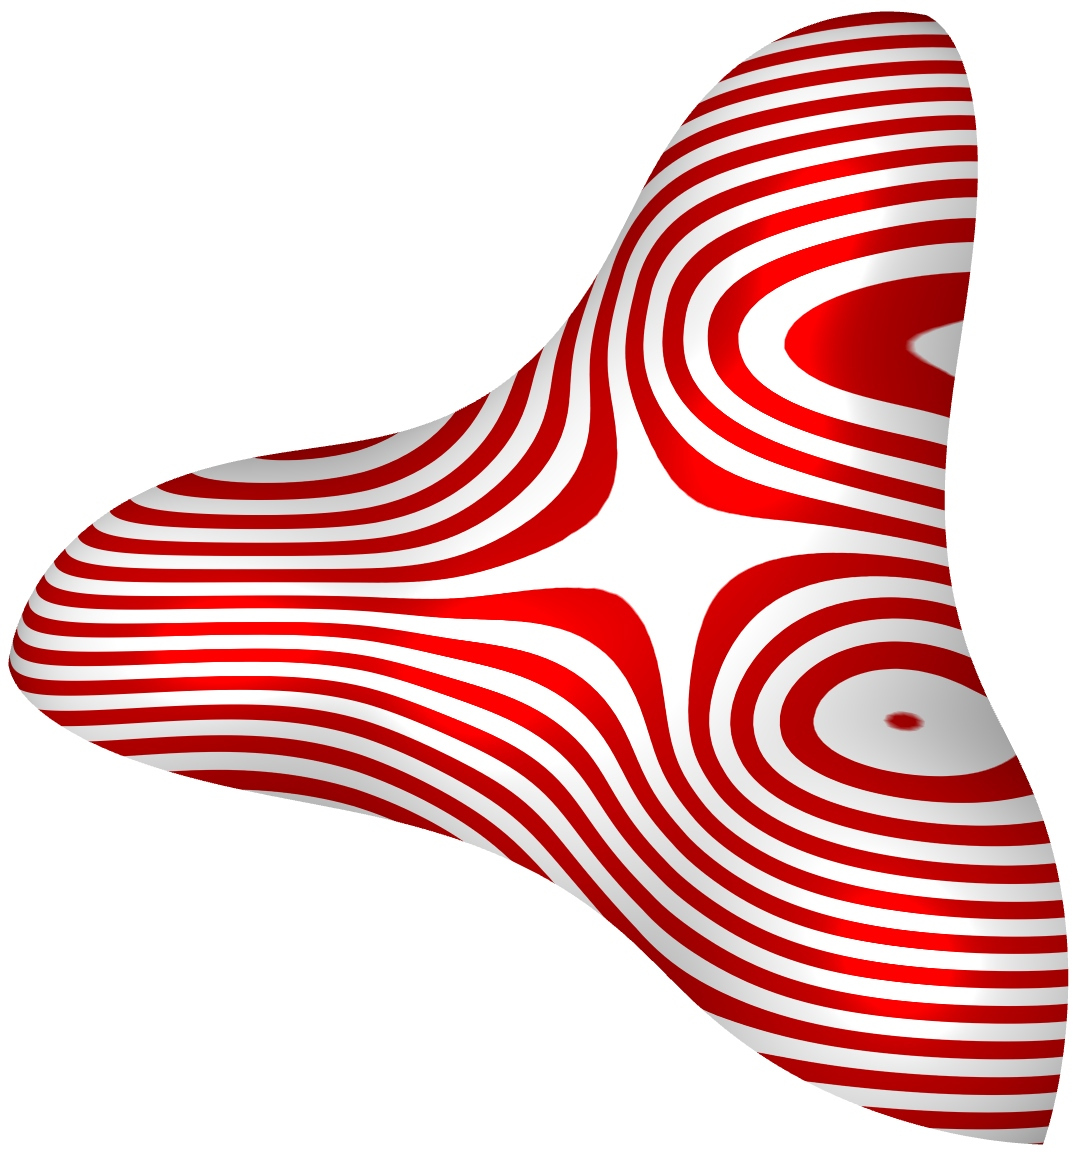
\includegraphics[width = 0.23\textwidth]{images/trebol3-zebra.jpg}
\end{figure}

\vspace{10pt}
\noindent\underline{Discussion:}\vspace{0.2em}\newline
One aspect of the tensor product conversion we have not touched on before is the \emph{quality}
of the control net. Aside from Warren's patch, which has singular control points,
all the other representations have singularities in or outside their domains.
When a singular point is close to the domain of the tensor product patch (i.e., the unit square),
the control points in the vicinity show erratic behavior.

Kato's patch is singular at the corner vertices, and the S-patch is singular on the circle that goes
through the intersections of the lines containing the domain edges; however, the Charrot--Gregory patch
is singular only at these intersection points. Practically this means that excluding the triangular
S-patch (which is not rational) and the Charrot--Gregory patch for $n\leq6$ (where singularities are
relatively far away), all of these converted tensor product surfaces are likely to have
badly oscillating control points (possibly tending to infinity), which may lead to numerical issues.

We present a solution to this problem. Normally the multi-sided domain is inside the unit
square (Figure~\ref{fig:parameters}), so that the trimming curves will be inside the
surface, but if we lift this constraint, we can create a larger multi-sided domain,
thereby separating the unit square from the singularities. This means that the actual ``trimmed''
region will be outside the standard $[0,1]^2$ domain; this may not be supported by some
applications, but the control structure will be close to the surface. The figure below shows
the control net of an 8-sided Charrot--Gregory patch with default and enlarged domain,
and isophote lines.
\begin{figure}[h!]
  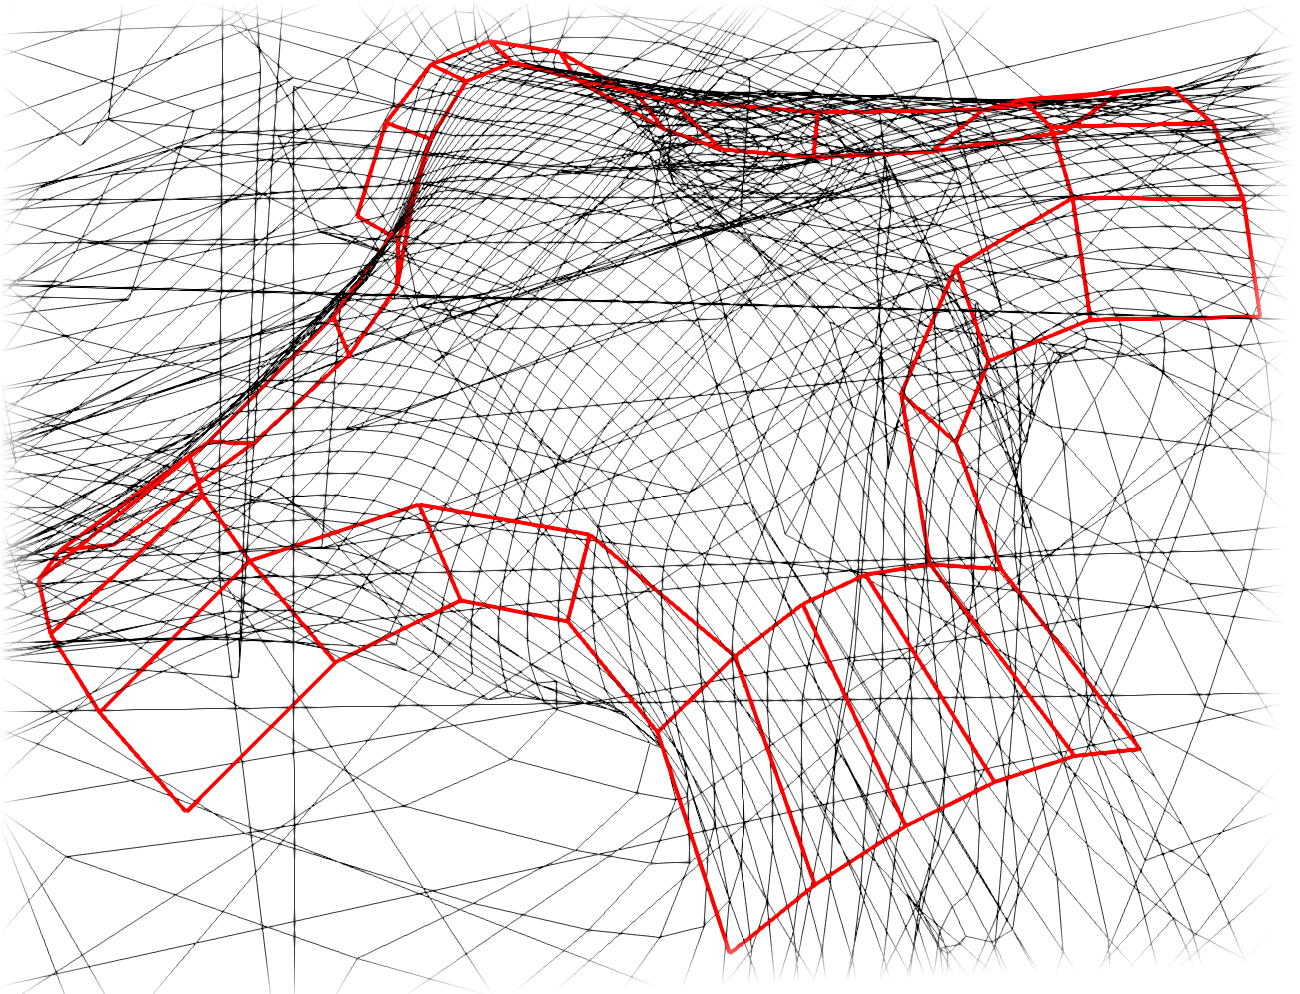
\includegraphics[width = 0.34\textwidth]{images/8sided-1.png}
  \hfill
  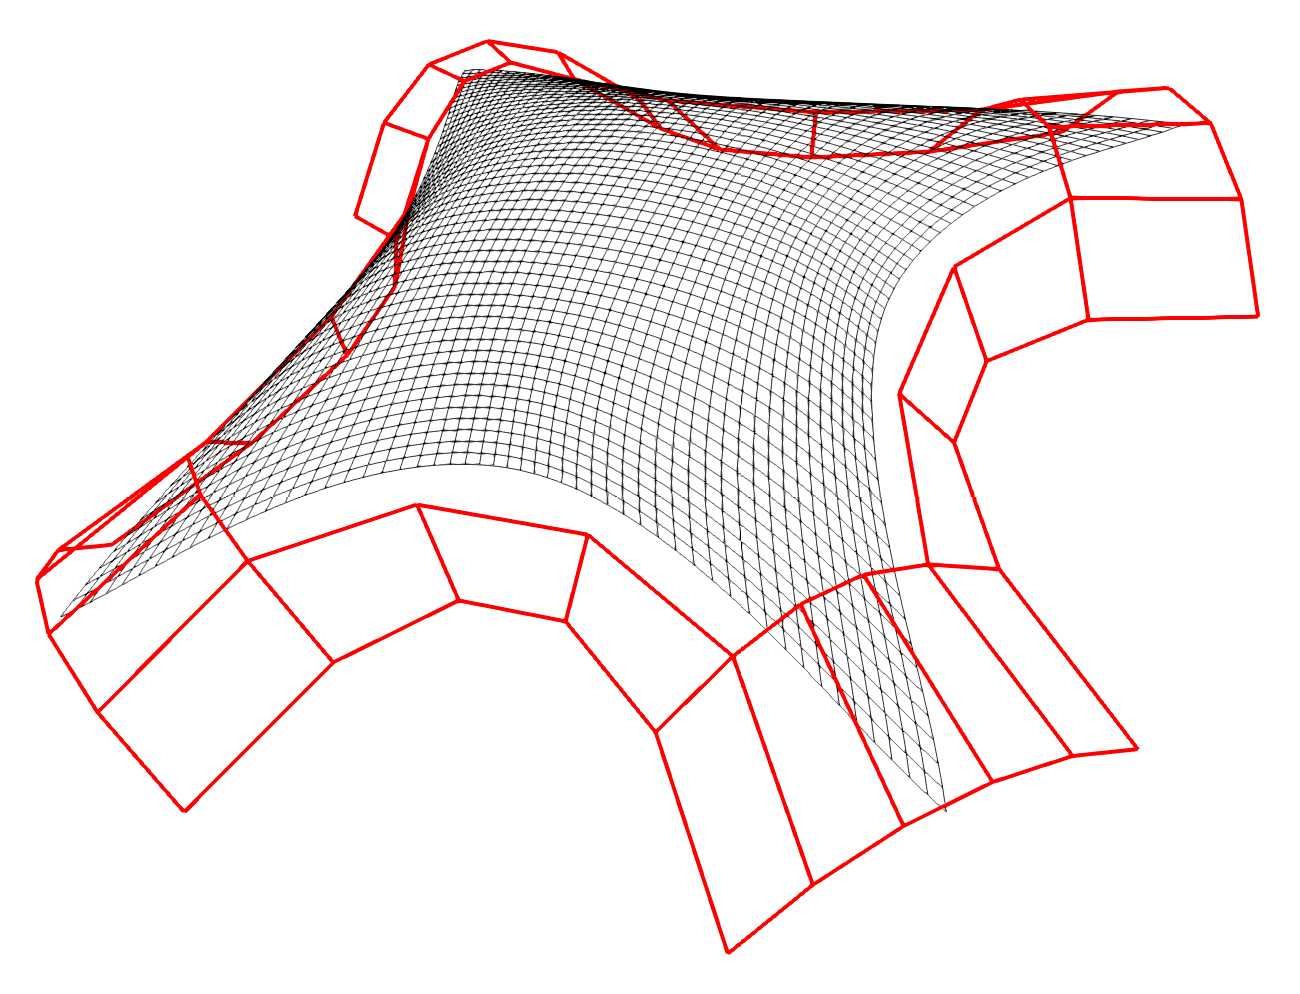
\includegraphics[width = 0.34\textwidth]{images/8sided-2.png}
  \hfill
  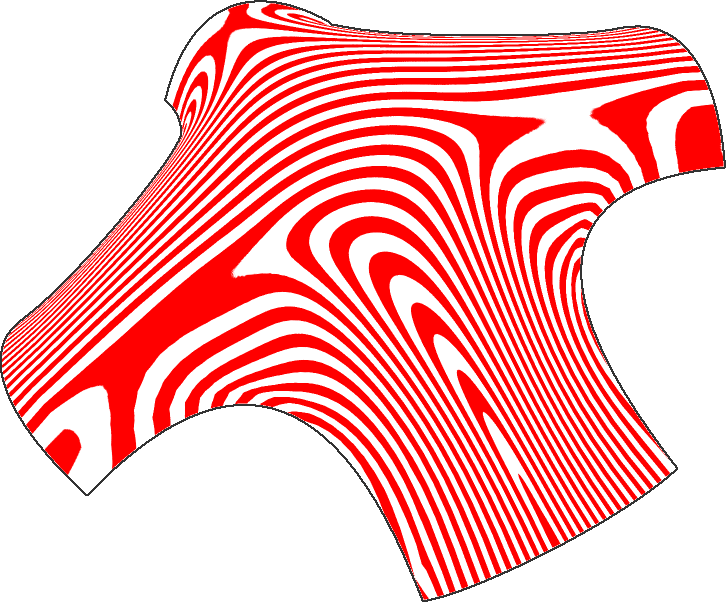
\includegraphics[width = 0.3\textwidth]{images/8sided-3.png}
\end{figure}

% Rotation
%% \begin{figure}[h!]
%%   \centering
%%   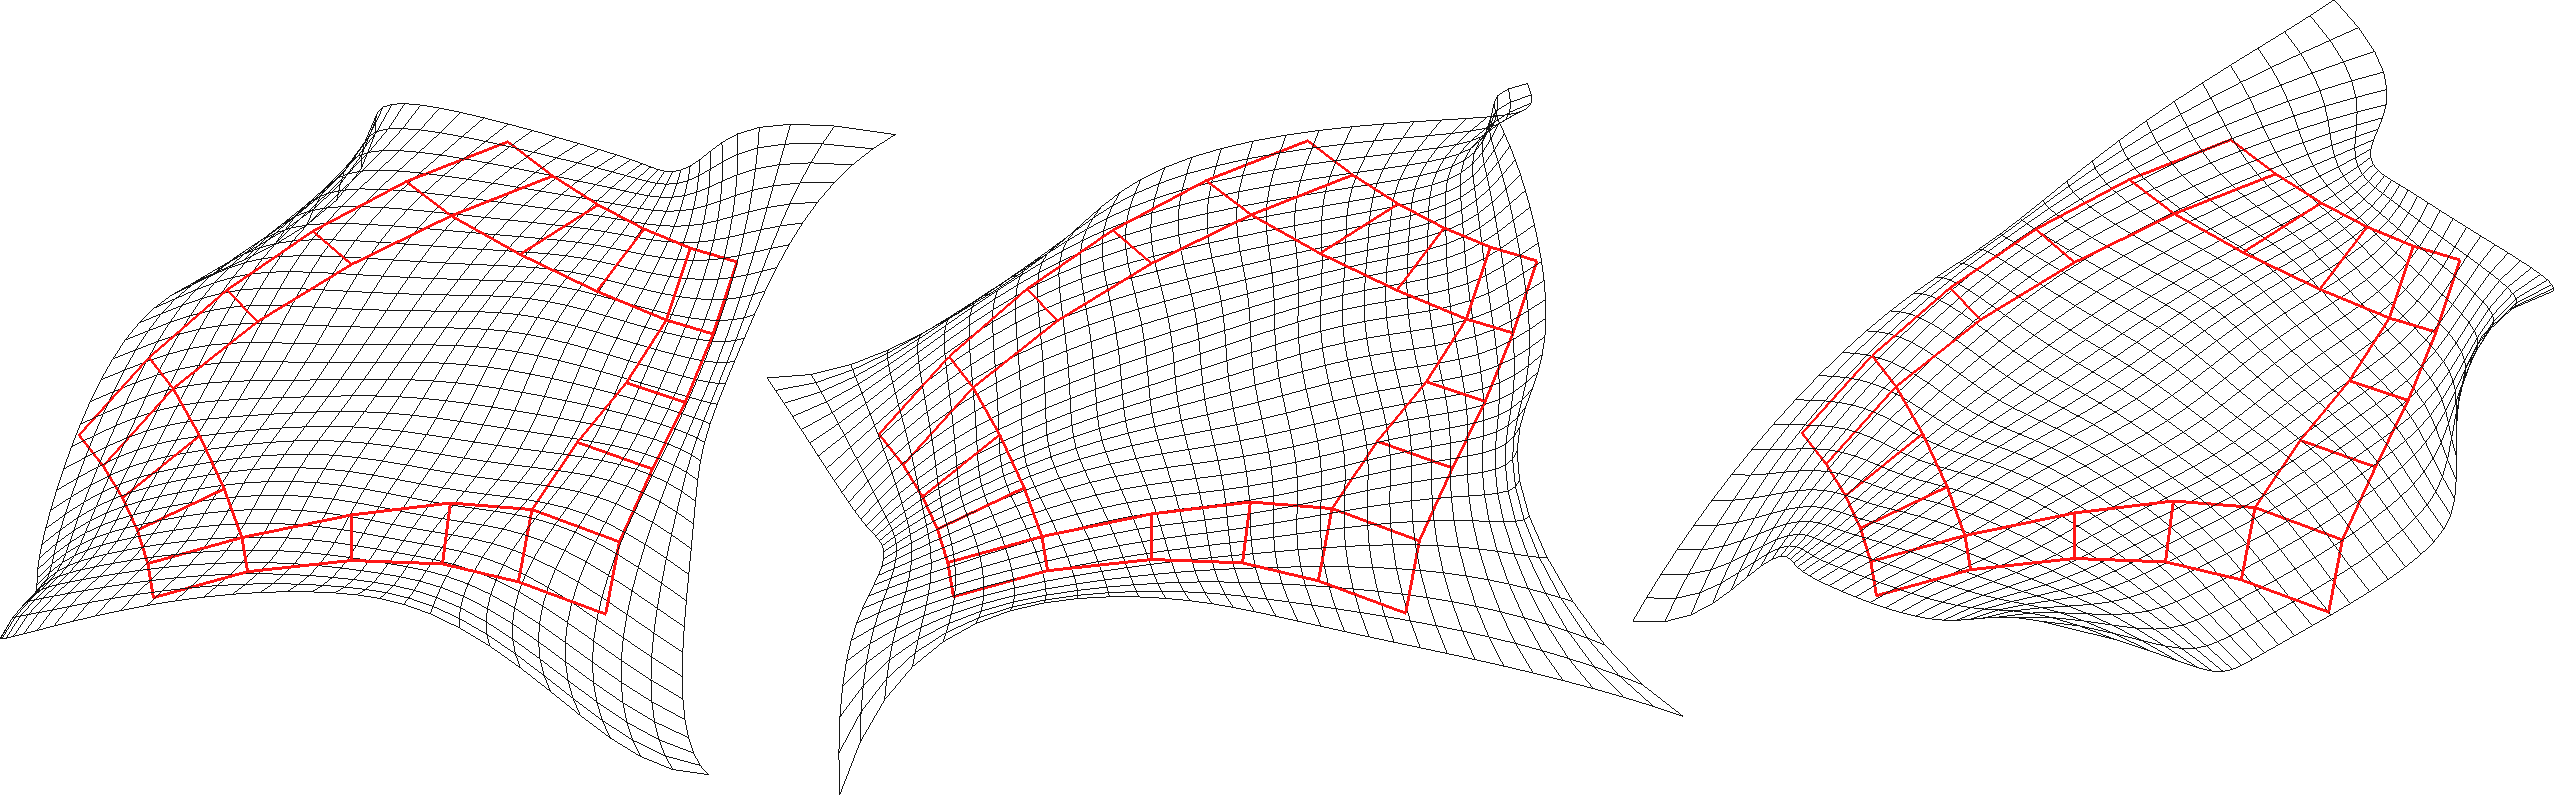
\includegraphics[width = 0.9\textwidth]{images/rotations.png}
%%   \caption{Effects of rotating the multi-sided domain.}
%%   \label{fig:rotations}
%% \end{figure}

\begin{table}
  \centering
  \begin{tabular}{c|c|c|c|c}
    $n$ & S-patch~\cite{spatch1} & Warren~\cite{warren} & Kato~\cite{kato} & Charrot--Gregory~\cite{charrot} \\ \hline
    3 & \multicolumn{2}{c|}{$d[+3]$ (both are B\'ezier triangles)} & \cellcolor{light-gray}$3d+5$ & $d+3$ \\ \hline
    5 & \cellcolor{light-light-gray}$3d[+9]$ & $\approx 3d$ & \cellcolor{light-gray}$5d+9$ & $5d+6$ \\ \hline
    6 & \cellcolor{light-light-gray}$4d[+12]$ & $3d$ & \cellcolor{light-gray}$6d+11$ & $6d+8$ \\ \hline
    7+ & \cellcolor{light-gray}$(n-2)(d[+3])$ & $\qquad$N/A$\qquad$ & \cellcolor{light-gray}$nd+2n-1$ & \cellcolor{light-gray}$nd+2n-4$ \\ \hline
  \end{tabular}
  \caption{Rational polynomial degrees of the converted surfaces for different number of sides,
    assuming boundary curves of degree $d$. Gray cells indicate that the surface is susceptible to
    the singularity issue.
    For S-patches, the number in brackets is applied
    when the surface is generated by a degree-$d$ $G^1$ frame.}
  \label{tab:degrees}
\end{table}

Table~\ref{tab:degrees} summarizes the degrees of all four representations.
% Note that triangular S-patches and Warren patches are both B\'ezier triangles.
It can be seen that these patches
have relatively high degrees, in particular when the number of sides and the degree of the
boundaries are raised. While Warren's patch outperforms the others in this respect,
the use of base points somewhat limits its usability in CAD systems.
Kato's surface always has singularities, and its degree is fairly high, but it is the only
construction where $G^2$ continuity can be easily achieved. We found that while the
Charrot--Gregory patch has a slightly higher degree than the S-patch, it has much lower
computational cost in its multi-sided form, and have no control net quality problems for 5-
and 6-sided configurations.

\vspace{10pt}
\noindent\underline{Conclusion:}\vspace{0.2em}\newline
In the full paper we are going to give representation details, and
further analyze the difficulties of the conversion process.
The computational efficiency of the proposed procedures
and the avoidance of wiggling control structures
will be the focal part of our discussion,
together with several comparative examples.

\vspace{1em}
\noindent\underline{Acknowledgment:}\vspace{0.2em}\newline
This project has been supported by the Hungarian Scientific Research Fund (OTKA, No.~124727).

\vspace{1em}
\noindent\underline{References:}\vspace{-1.9em}\newline
\renewcommand{\section}[2]{}
\begin{thebibliography}{99}

\bibitem{charrot} Charrot, P.; Gregory, J.~A.: A pentagonal surface patch for computer aided geometric design, Computer Aided Geometric Design, 1(1), 1984, 87--94.\\\ULurl{https://doi.org/10.1016/0167-8396(84)90006-2}
%\bibitem{simplex1} DeRose, T.~D.: Composing B\'ezier simplexes, ACM Transactions on Graphics, 7(3), 1988, 198--221.\\\ULurl{https://doi.org/10.1145/44479.44482}
\bibitem{simplex2} DeRose, T.~D.; Goldman, R.~N.; Hagen, H.; Mann, S.: Functional composition algorithms via blossoming, ACM Transactions on Graphics, 12(2), 1993, 113--135.\\\ULurl{https://doi.org/10.1145/151280.151290}
%\bibitem{floater} Floater, M.~S.: Generalized barycentric coordinates and applications, Acta Numerica, 24, 2015, 161--214.
\bibitem{kato} Kato, K.: Generation of $n$-sided surface patches with holes, Computer-Aided Design, 23(10), 1991, 676--683. \ULurl{https://doi.org/10.1016/0010-4485(91)90020-W}
%\bibitem{toric} Krasauskas, R.: Toric surface patches, Advances in Computational Mathematics, 17(1), 2002, 89--113. \ULurl{https://doi.org/10.1023/A:1015289823859}
\bibitem{spatch1} Loop, Ch.~T.; DeRose, T.~D.: A multisided generalization of B\'ezier surfaces, ACM Transactions on Graphics, 8(3), 1989, 204--234. \ULurl{https://doi.org/10.1145/77055.77059}
\bibitem{spatch2} Loop, Ch.~T.; DeRose, T.~D.: Generalized B-spline surfaces of arbitrary topology, ACM, 17th Conference on Computer Graphics and Interactive Techniques, 1990, 347--356.\\\ULurl{https://doi.org/10.1145/97879.97917}
\bibitem{salvi-kepaf} Salvi, P.: $G^1$ hole filling with S-patches made easy, Proceedings of the 12th Conference of the Hungarian Association for Image Processing and Pattern Recognition, 2019, 1--8.
\bibitem{salvi-wait} Salvi, P.: On the CAD-compatible conversion of S-patches, Proceedings of the Workshop on the Advances of Information Technology, 2019, 72--76.
%\bibitem{transfinite} V\'arady, T.; Rockwood, A.; Salvi, P.: Transfinite surface interpolation over irregular $n$-sided domains, Computer-Aided Design, 43(11), 2011, 1330--1340. \ULurl{https://doi.org/10.1016/j.cad.2011.08.028}
\bibitem{warren} Warren, J.: Creating multisided rational B\'ezier surfaces using base points, ACM Transactions on Graphics, 11(2), 1992, 127--139. \ULurl{https://doi.org/10.1145/130826.130828}

\end{thebibliography}

\end{document}
